% Options for packages loaded elsewhere
% Options for packages loaded elsewhere
\PassOptionsToPackage{unicode}{hyperref}
\PassOptionsToPackage{hyphens}{url}
\PassOptionsToPackage{dvipsnames,svgnames,x11names}{xcolor}
%
\documentclass[
  12pt,
  letterpaper,
]{scrreprt}
\usepackage{xcolor}
\usepackage{amsmath,amssymb}
\setcounter{secnumdepth}{3}
\usepackage{iftex}
\ifPDFTeX
  \usepackage[T1]{fontenc}
  \usepackage[utf8]{inputenc}
  \usepackage{textcomp} % provide euro and other symbols
\else % if luatex or xetex
  \usepackage{unicode-math} % this also loads fontspec
  \defaultfontfeatures{Scale=MatchLowercase}
  \defaultfontfeatures[\rmfamily]{Ligatures=TeX,Scale=1}
\fi
\usepackage{lmodern}
\ifPDFTeX\else
  % xetex/luatex font selection
  \setmainfont[]{Times New Roman}
  \setsansfont[]{Times New Roman}
\fi
% Use upquote if available, for straight quotes in verbatim environments
\IfFileExists{upquote.sty}{\usepackage{upquote}}{}
\IfFileExists{microtype.sty}{% use microtype if available
  \usepackage[]{microtype}
  \UseMicrotypeSet[protrusion]{basicmath} % disable protrusion for tt fonts
}{}
\usepackage{setspace}
\makeatletter
\@ifundefined{KOMAClassName}{% if non-KOMA class
  \IfFileExists{parskip.sty}{%
    \usepackage{parskip}
  }{% else
    \setlength{\parindent}{0pt}
    \setlength{\parskip}{6pt plus 2pt minus 1pt}}
}{% if KOMA class
  \KOMAoptions{parskip=half}}
\makeatother
% Make \paragraph and \subparagraph free-standing
\makeatletter
\ifx\paragraph\undefined\else
  \let\oldparagraph\paragraph
  \renewcommand{\paragraph}{
    \@ifstar
      \xxxParagraphStar
      \xxxParagraphNoStar
  }
  \newcommand{\xxxParagraphStar}[1]{\oldparagraph*{#1}\mbox{}}
  \newcommand{\xxxParagraphNoStar}[1]{\oldparagraph{#1}\mbox{}}
\fi
\ifx\subparagraph\undefined\else
  \let\oldsubparagraph\subparagraph
  \renewcommand{\subparagraph}{
    \@ifstar
      \xxxSubParagraphStar
      \xxxSubParagraphNoStar
  }
  \newcommand{\xxxSubParagraphStar}[1]{\oldsubparagraph*{#1}\mbox{}}
  \newcommand{\xxxSubParagraphNoStar}[1]{\oldsubparagraph{#1}\mbox{}}
\fi
\makeatother

\usepackage{color}
\usepackage{fancyvrb}
\newcommand{\VerbBar}{|}
\newcommand{\VERB}{\Verb[commandchars=\\\{\}]}
\DefineVerbatimEnvironment{Highlighting}{Verbatim}{commandchars=\\\{\}}
% Add ',fontsize=\small' for more characters per line
\usepackage{framed}
\definecolor{shadecolor}{RGB}{241,243,245}
\newenvironment{Shaded}{\begin{snugshade}}{\end{snugshade}}
\newcommand{\AlertTok}[1]{\textcolor[rgb]{0.68,0.00,0.00}{#1}}
\newcommand{\AnnotationTok}[1]{\textcolor[rgb]{0.37,0.37,0.37}{#1}}
\newcommand{\AttributeTok}[1]{\textcolor[rgb]{0.40,0.45,0.13}{#1}}
\newcommand{\BaseNTok}[1]{\textcolor[rgb]{0.68,0.00,0.00}{#1}}
\newcommand{\BuiltInTok}[1]{\textcolor[rgb]{0.00,0.23,0.31}{#1}}
\newcommand{\CharTok}[1]{\textcolor[rgb]{0.13,0.47,0.30}{#1}}
\newcommand{\CommentTok}[1]{\textcolor[rgb]{0.37,0.37,0.37}{#1}}
\newcommand{\CommentVarTok}[1]{\textcolor[rgb]{0.37,0.37,0.37}{\textit{#1}}}
\newcommand{\ConstantTok}[1]{\textcolor[rgb]{0.56,0.35,0.01}{#1}}
\newcommand{\ControlFlowTok}[1]{\textcolor[rgb]{0.00,0.23,0.31}{\textbf{#1}}}
\newcommand{\DataTypeTok}[1]{\textcolor[rgb]{0.68,0.00,0.00}{#1}}
\newcommand{\DecValTok}[1]{\textcolor[rgb]{0.68,0.00,0.00}{#1}}
\newcommand{\DocumentationTok}[1]{\textcolor[rgb]{0.37,0.37,0.37}{\textit{#1}}}
\newcommand{\ErrorTok}[1]{\textcolor[rgb]{0.68,0.00,0.00}{#1}}
\newcommand{\ExtensionTok}[1]{\textcolor[rgb]{0.00,0.23,0.31}{#1}}
\newcommand{\FloatTok}[1]{\textcolor[rgb]{0.68,0.00,0.00}{#1}}
\newcommand{\FunctionTok}[1]{\textcolor[rgb]{0.28,0.35,0.67}{#1}}
\newcommand{\ImportTok}[1]{\textcolor[rgb]{0.00,0.46,0.62}{#1}}
\newcommand{\InformationTok}[1]{\textcolor[rgb]{0.37,0.37,0.37}{#1}}
\newcommand{\KeywordTok}[1]{\textcolor[rgb]{0.00,0.23,0.31}{\textbf{#1}}}
\newcommand{\NormalTok}[1]{\textcolor[rgb]{0.00,0.23,0.31}{#1}}
\newcommand{\OperatorTok}[1]{\textcolor[rgb]{0.37,0.37,0.37}{#1}}
\newcommand{\OtherTok}[1]{\textcolor[rgb]{0.00,0.23,0.31}{#1}}
\newcommand{\PreprocessorTok}[1]{\textcolor[rgb]{0.68,0.00,0.00}{#1}}
\newcommand{\RegionMarkerTok}[1]{\textcolor[rgb]{0.00,0.23,0.31}{#1}}
\newcommand{\SpecialCharTok}[1]{\textcolor[rgb]{0.37,0.37,0.37}{#1}}
\newcommand{\SpecialStringTok}[1]{\textcolor[rgb]{0.13,0.47,0.30}{#1}}
\newcommand{\StringTok}[1]{\textcolor[rgb]{0.13,0.47,0.30}{#1}}
\newcommand{\VariableTok}[1]{\textcolor[rgb]{0.07,0.07,0.07}{#1}}
\newcommand{\VerbatimStringTok}[1]{\textcolor[rgb]{0.13,0.47,0.30}{#1}}
\newcommand{\WarningTok}[1]{\textcolor[rgb]{0.37,0.37,0.37}{\textit{#1}}}

\usepackage{longtable,booktabs,array}
\newcounter{none} % for unnumbered tables
\usepackage{calc} % for calculating minipage widths
% Correct order of tables after \paragraph or \subparagraph
\usepackage{etoolbox}
\makeatletter
\patchcmd\longtable{\par}{\if@noskipsec\mbox{}\fi\par}{}{}
\makeatother
% Allow footnotes in longtable head/foot
\IfFileExists{footnotehyper.sty}{\usepackage{footnotehyper}}{\usepackage{footnote}}
\makesavenoteenv{longtable}
\usepackage{graphicx}
\makeatletter
\newsavebox\pandoc@box
\newcommand*\pandocbounded[1]{% scales image to fit in text height/width
  \sbox\pandoc@box{#1}%
  \Gscale@div\@tempa{\textheight}{\dimexpr\ht\pandoc@box+\dp\pandoc@box\relax}%
  \Gscale@div\@tempb{\linewidth}{\wd\pandoc@box}%
  \ifdim\@tempb\p@<\@tempa\p@\let\@tempa\@tempb\fi% select the smaller of both
  \ifdim\@tempa\p@<\p@\scalebox{\@tempa}{\usebox\pandoc@box}%
  \else\usebox{\pandoc@box}%
  \fi%
}
% Set default figure placement to htbp
\def\fps@figure{htbp}
\makeatother





\setlength{\emergencystretch}{3em} % prevent overfull lines

\providecommand{\tightlist}{%
  \setlength{\itemsep}{0pt}\setlength{\parskip}{0pt}}



 


% preamble_custom.tex — only for header inclusion
\usepackage{graphicx}
\usepackage{float}
\usepackage[section]{placeins} % auto \FloatBarrier before each \section
\usepackage{parskip}
\usepackage{setspace}
\usepackage{fontspec} % Required for xelatex
\setmainfont{Times New Roman}
\usepackage{xcolor}
\usepackage{multicol}
\usepackage{zref}
\usepackage{atbegshi}
\usepackage{etoolbox}
\usepackage{color}
\setstretch{1.5}
\usepackage{pdfpages}
\usepackage{fontspec}
\newfontfamily\hindifont{Aparajita}
\usepackage{longtable}
\usepackage{bookmark}
\usepackage{hyperref}
\makeatletter
\patchcmd{\@sect}{\@mkboth}{{\thispagestyle{empty}}\@mkboth}{}{}
\makeatother
\pagenumbering{roman}

\usepackage{tikz}
\usepackage{atbegshi}

\definecolor{aiimsolive}{RGB}{85,107,47}
\AtBeginShipout{%
  \AtBeginShipoutUpperLeft{%
    \begin{tikzpicture}[remember picture, overlay]
      \draw[color=aiimsolive,line width=2pt]
        ([xshift=0.55in, yshift=-0.6in]current page.north west) rectangle
        ([xshift=-0.5in, yshift=0.7in]current page.south east);
    \end{tikzpicture}
  }
}

\usepackage[
  a4paper,
  top=1.1in,
  bottom=1.1in,
  left=1.1in,
  right=1.1in,
  footskip=0.5in
]{geometry}
\pagestyle{empty}

\AtBeginShipout{%
  \ifnum\value{page}>1
    \AtBeginShipoutUpperLeft{%
      \begin{tikzpicture}[remember picture, overlay]
        \node[anchor=south, font=\normalfont]
          at ([xshift=0.5\paperwidth, yshift=0.8cm]current page.south west)
          {\thepage};
      \end{tikzpicture}
    }%
  \fi
}

\makeatletter
\pretocmd{\@chapter}{\thispagestyle{empty}}{}{}
\makeatother

\makeatletter
\let\ps@plain\ps@empty
\makeatother
% chapter-top-offset.tex
% Purpose:
% Set the vertical starting position of every level-one heading in a
% Quarto PDF that uses the KOMA-Script scrreprt document class.
%
% In scrreprt, Quarto/Pandoc converts level-one headings into \chapter.
% KOMA-Script inserts its own vertical space before each chapter heading.
% Changing \chapterheadstartvskip therefore controls that space directly,
% without replacing or reconstructing the heading.
%
% The starred form of \vspace preserves the 1 cm space at the top of a page.
% The distance is measured downward from the top of the text area (the top
% margin boundary), not from the physical top edge of the paper.
%
% This leaves chapter numbering, appendix labels, table-of-contents entries,
% bookmarks, identifiers, cross-references, colours, and alignment unchanged.
%
% Requirement: documentclass: scrreprt

\renewcommand*{\chapterheadstartvskip}{\vspace*{-0.2cm}}
\makeatletter
\@ifpackageloaded{bookmark}{}{\usepackage{bookmark}}
\makeatother
\makeatletter
\@ifpackageloaded{caption}{}{\usepackage{caption}}
\AtBeginDocument{%
\ifdefined\contentsname
  \renewcommand*\contentsname{Table of contents}
\else
  \newcommand\contentsname{Table of contents}
\fi
\ifdefined\listfigurename
  \renewcommand*\listfigurename{List of Figures}
\else
  \newcommand\listfigurename{List of Figures}
\fi
\ifdefined\listtablename
  \renewcommand*\listtablename{List of Tables}
\else
  \newcommand\listtablename{List of Tables}
\fi
\ifdefined\figurename
  \renewcommand*\figurename{Figure}
\else
  \newcommand\figurename{Figure}
\fi
\ifdefined\tablename
  \renewcommand*\tablename{Table}
\else
  \newcommand\tablename{Table}
\fi
}
\@ifpackageloaded{float}{}{\usepackage{float}}
\floatstyle{ruled}
\@ifundefined{c@chapter}{\newfloat{codelisting}{h}{lop}}{\newfloat{codelisting}{h}{lop}[chapter]}
\floatname{codelisting}{Listing}
\newcommand*\listoflistings{\listof{codelisting}{List of Listings}}
\makeatother
\makeatletter
\usepackage{pdflscape}
\makeatother
\makeatletter
\makeatother
\makeatletter
\@ifpackageloaded{caption}{}{\usepackage{caption}}
\@ifpackageloaded{subcaption}{}{\usepackage{subcaption}}
\makeatother
\usepackage{bookmark}
\IfFileExists{xurl.sty}{\usepackage{xurl}}{} % add URL line breaks if available
\urlstyle{same}
\hypersetup{
  pdftitle={Estimation Of Prevalence And Factors Associated With Developmental Delay In Under Five Children Residing In Selected Urban Slums Of Patna: A Community Based Cross Sectional Study},
  pdfauthor={Dr.~Naveen Suthar},
  colorlinks=true,
  linkcolor={blue},
  filecolor={Maroon},
  citecolor={Blue},
  urlcolor={Blue},
  pdfcreator={LaTeX via pandoc}}


% partials/title.tex  (single-page, contained title page)

\def\maketitle{%
  \thispagestyle{empty}%
 \begingroup
\setstretch{1.2}
\def\gapS{\vskip 0.4cm plus 1fill}
\def\gapM{\vskip 0.6cm plus 2fill}
\def\gapL{\vskip 1cm plus 3fill}


  \vbox to \textheight{%
    \vfil
    \begin{center}
      \begin{minipage}{0.90\textwidth}
        \centering

        % Logo (make sure filename matches extension resource)
% inside minipage after \centering

\includegraphics[width=2.2in]{aiims_patna_logo.jpeg}

\gapL
{\LARGE\bfseries Estimation Of Prevalence And Factors Associated With
Developmental Delay In Under Five Children Residing In Selected Urban
Slums Of Patna: A Community Based Cross Sectional Study \par}

\gapM
{\large THESIS SUBMITTED IN PARTIAL FULFILLMENT OF THE REQUIREMENT FOR THE AWARD OF THE DEGREE OF\par}

\gapM
{\fontsize{16}{20}\selectfont\bfseries MD \par}
{\fontsize{16}{20}\selectfont\bfseries (Community And Family
Medicine)\par}

\gapM
{\fontsize{14}{18}\selectfont\bfseries Under\par}
{\fontsize{14}{18}\selectfont\bfseries All India Institute of Medical
Sciences, Patna\par}
{\fontsize{14}{18}\selectfont\bfseries (SESSION: January 2023 -- January
2026)\par}

\gapM
{\fontsize{14}{18}\selectfont\bfseries By\par}
{\fontsize{14}{18}\selectfont\bfseries Dr.~Naveen Suthar \par}
{\fontsize{14}{18}\selectfont\bfseries Department of Community And
Family Medicine\par}
{\fontsize{14}{18}\selectfont\bfseries All India Institute of Medical
Sciences, Patna\par}
      \end{minipage}
    \end{center}
    \vfil
  }%
 \endgroup
  \clearpage
}

\title{Estimation Of Prevalence And Factors Associated With
Developmental Delay In Under Five Children Residing In Selected Urban
Slums Of Patna: A Community Based Cross Sectional Study}



\begin{document}
\maketitle


\setstretch{1.5}
\bookmarksetup{startatroot}

\chapter*{Declaration By HOD}\label{declaration-by-hod}
\addcontentsline{toc}{chapter}{Declaration By HOD}

\markboth{Declaration By HOD}{Declaration By HOD}

\begin{center}
  
\includegraphics[width=1.8in]{aiims_patna_logo.jpeg}\par
  \vspace{1em}
  {\Large\bfseries All India Institute of Medical Sciences, Patna\par}
\end{center}

\vspace{1em}

This is to certify that \textbf{ Dr. Naveen Suthar }, is a postgraduate
resident of MD Community And Family Medicine course for the session
January 2023 -- January 2026, and he has independantly carried out this
thesis entitled
\textbf{ “ Estimation Of Prevalence And Factors Associated With Developmental Delay In Under Five Children Residing In Selected Urban Slums Of Patna: A Community Based Cross Sectional Study ” }
for MD in Community And Family Medicine of the All India Institute of
Medical Sciences, Patna in the Department of Community And Family
Medicine, under the guidance of Dr Guide Name .

\vfill

\begin{center}

\includegraphics[width=2.2in, angle=180]{assets/sign.png}\par
\textbf{ Dr HOD Name  }\par
Professor and Head of Department \par
Department of Community And Family Medicine \par
AIIMS Patna
\end{center}

\vfill

\noindent Date: today

\par

\noindent Place: All India Institute of Medical Sciences Patna

\bookmarksetup{startatroot}

\chapter*{Declaration By Guide}\label{declaration-by-guide}
\addcontentsline{toc}{chapter}{Declaration By Guide}

\markboth{Declaration By Guide}{Declaration By Guide}

\begin{center}
  
\includegraphics[width=1.8in]{aiims_patna_logo.jpeg}\par
  \vspace{1em}
  {\Large\bfseries All India Institute of Medical Sciences, Patna\par}
\end{center}

\vspace{2em}

I hereby declare that this thesis work entitled
\textbf{ “ Estimation Of Prevalence And Factors Associated With Developmental Delay In Under Five Children Residing In Selected Urban Slums Of Patna: A Community Based Cross Sectional Study ” },
which is being submitted as a requirement for the award of the MD degree
in the subject of Community And Family Medicine , is a bonafide work of
the Postgraduate student \textbf{ Dr. Naveen Suthar } of All India
Institute of Medical Sciences, Patna. This thesis work is carried out
under our constant supervision and guidance and to my full satisfaction.

\vfill

\begin{center}
  \vspace{0.5em}
\textbf{ Dr Guide Name  }\par
Professor \par
Department of Community And Family Medicine \par
AIIMS Patna
\end{center}

\vfill

\noindent Date: today

\par

\noindent Place: All India Institute of Medical Sciences Patna

\bookmarksetup{startatroot}

\chapter*{Declaration by Coguides}\label{declaration-by-coguides}
\addcontentsline{toc}{chapter}{Declaration by Coguides}

\markboth{Declaration by Coguides}{Declaration by Coguides}

\begin{center}
  
\includegraphics[width=1.8in]{aiims_patna_logo.jpeg}\par
  \vspace{1em}
  {\Large\bfseries All India Institute of Medical Sciences, Patna\par}
\end{center}

\vspace{2em}

I hereby declare that this thesis work entitled
\textbf{ “ Estimation Of Prevalence And Factors Associated With Developmental Delay In Under Five Children Residing In Selected Urban Slums Of Patna: A Community Based Cross Sectional Study ” },
which is being submitted as a requirement for the award of the MD degree
in the subject of Community And Family Medicine , is a bonafide work of
the Postgraduate student \textbf{ Dr. Naveen Suthar } of All India
Institute of Medical Sciences, Patna. This thesis work is carried out
under our constant supervision and guidance and to our full
satisfaction.

\vfill

{\def\LTcaptype{none} % do not increment counter
\begin{longtable}[]{@{}
  >{\raggedright\arraybackslash}p{(\linewidth - 4\tabcolsep) * \real{0.3750}}
  >{\raggedright\arraybackslash}p{(\linewidth - 4\tabcolsep) * \real{0.2500}}
  >{\raggedright\arraybackslash}p{(\linewidth - 4\tabcolsep) * \real{0.3750}}@{}}
\toprule\noalign{}
\endhead
\bottomrule\noalign{}
\endlastfoot
\textbf{ Dr Co-Guide 1 Name } & & \textbf{  Dr Co-Guide 2 Name  } \\
Professor & & Professor \\
\textbf{?meta:coguide1.department} & &
\textbf{?meta:coguide2.department} \\
AIIMS Patna & & AIIMS Patna \\
\end{longtable}
}

\begin{center}

  \vspace{0.5em}
\end{center}

\vfill

\noindent Date: today

\par

\noindent Place: All India Institute of Medical Sciences Patna

\bookmarksetup{startatroot}

\chapter*{Declaration By Candidate}\label{declaration-by-candidate}
\addcontentsline{toc}{chapter}{Declaration By Candidate}

\markboth{Declaration By Candidate}{Declaration By Candidate}

\begin{center}
  
\includegraphics[width=1.8in]{aiims_patna_logo.jpeg}\par
  \vspace{1em}
  {\Large\bfseries All India Institute of Medical Sciences, Patna\par}
\end{center}

\vspace{2em}

I hereby declare that this thesis work entitled
\textbf{ “ Estimation Of Prevalence And Factors Associated With Developmental Delay In Under Five Children Residing In Selected Urban Slums Of Patna: A Community Based Cross Sectional Study ” },
submitted in the partial fulfillment of the requirement for the award of
the degree MD in the subject of Community And Family Medicine , All
India Institute of Medical Sciences, Patna, is a record of original work
done by me under the supervision of Dr Guide Name. The information and
data given in this research work is authenticated to the best of my
knowledge. This research is not submitted to any other university or
institution for the award of any degree, diploma, fellowship or
published any time before.

\vfill

\begin{center}
  \vspace{0.5em}
  
\includegraphics[width=4cm, angle=180]{assets/sign.png} \par
\textbf{ Dr. Naveen Suthar  }\par
January 2023 – January 2026 \par

\end{center}

\vfill

\noindent Date: today

\par

\noindent Place: All India Institute of Medical Sciences Patna

\bookmarksetup{startatroot}

\chapter*{IEC Approval}\label{iec-approval}
\addcontentsline{toc}{chapter}{IEC Approval}

\markboth{IEC Approval}{IEC Approval}

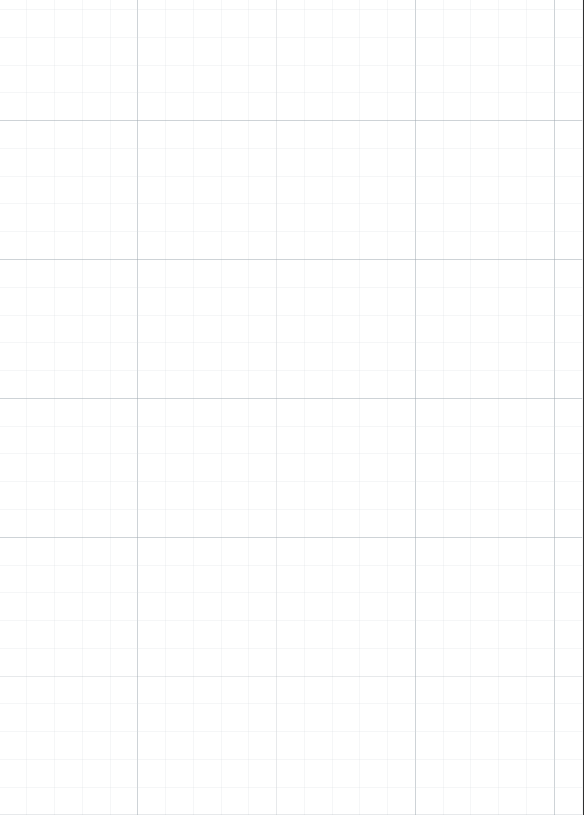
\includegraphics[width=0.95\linewidth,height=\textheight,keepaspectratio]{images/iec-front.png}

\newpage{}

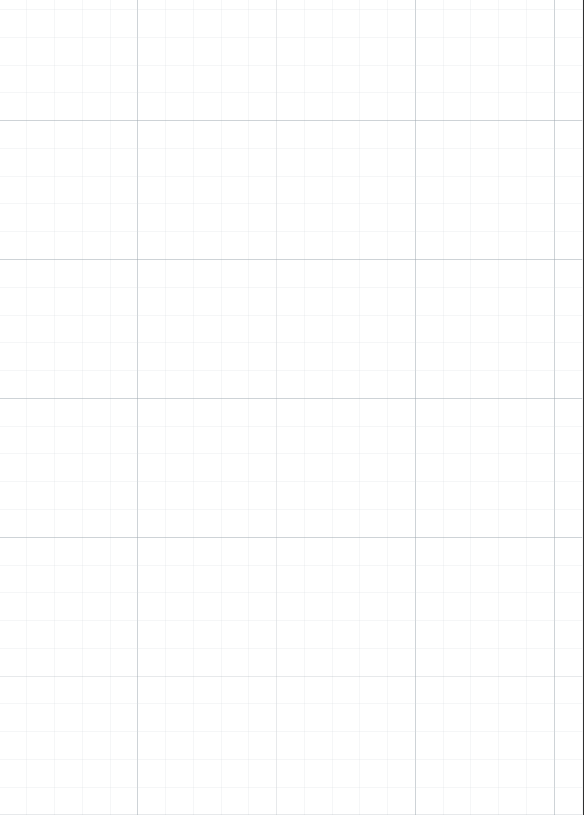
\includegraphics[width=0.95\linewidth,height=\textheight,keepaspectratio]{images/iec-back.png}

\bookmarksetup{startatroot}

\chapter*{PGMRC Approval}\label{pgmrc-approval}
\addcontentsline{toc}{chapter}{PGMRC Approval}

\markboth{PGMRC Approval}{PGMRC Approval}

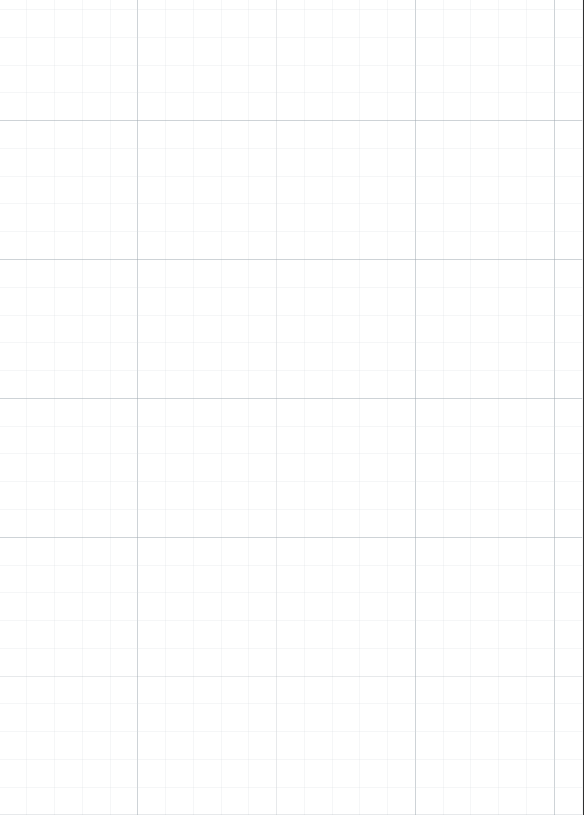
\includegraphics[width=0.95\linewidth,height=\textheight,keepaspectratio]{images/rac-front.png}

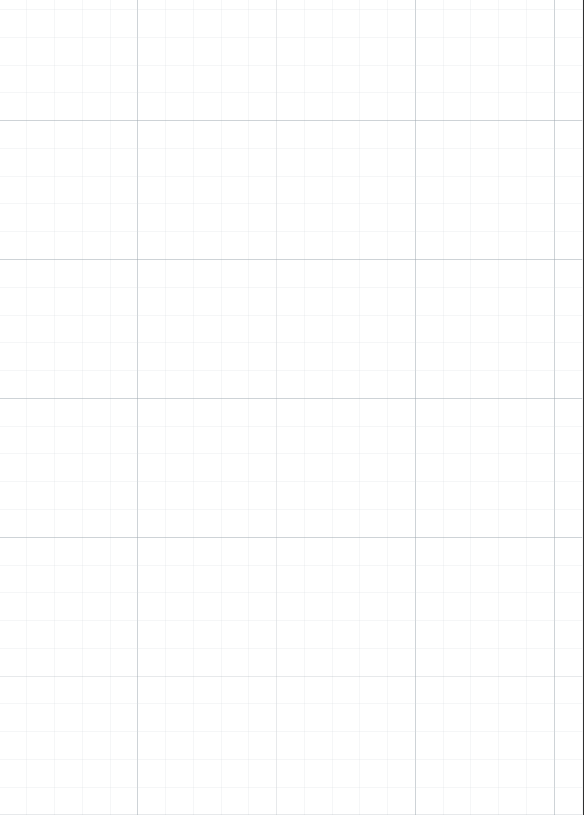
\includegraphics[width=0.95\linewidth,height=\textheight,keepaspectratio]{images/rac-back.png}

\bookmarksetup{startatroot}

\chapter*{Plagiarisum Check Report}\label{plagiarisum-check-report}
\addcontentsline{toc}{chapter}{Plagiarisum Check Report}

\markboth{Plagiarisum Check Report}{Plagiarisum Check Report}

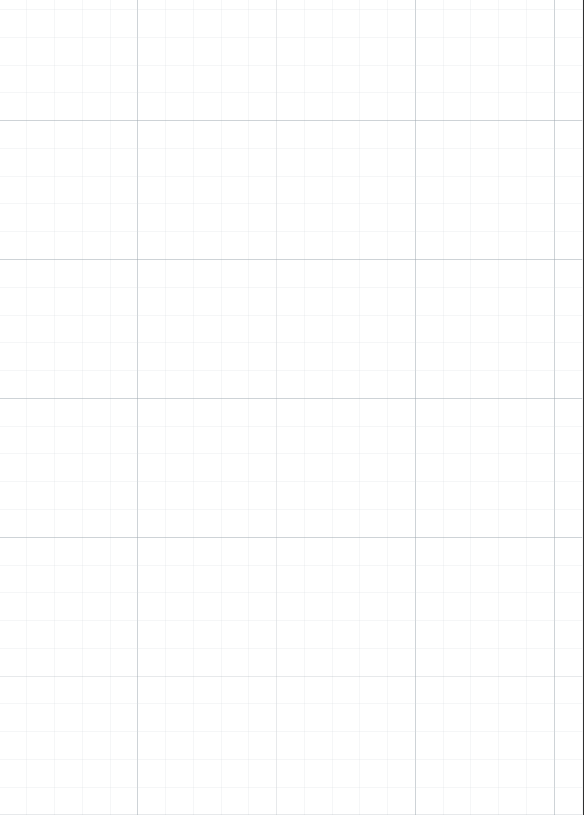
\includegraphics[width=0.95\linewidth,height=\textheight,keepaspectratio]{images/palgiarisum.png}

\bookmarksetup{startatroot}

\chapter*{Acknowledgement}\label{acknowledgement}
\addcontentsline{toc}{chapter}{Acknowledgement}

\markboth{Acknowledgement}{Acknowledgement}

I am eternally grateful to lord Jaggannath for constant Guidance and
Love.

This is Index file. This is a must file in book project.

It is a better Idea that we use this file for:

\begin{itemize}
\item
  Acknowledgement
\item
  Putting div for lua filter for list of abbreviations.
\item
  May be putting div for lua filter for certificates ? and toc ? lot?
  lof?
\end{itemize}

\hrulefill

\bookmarksetup{startatroot}

\chapter*{List of Abbreviations}\label{list-of-abbreviations}
\addcontentsline{toc}{chapter}{List of Abbreviations}

\markboth{List of Abbreviations}{List of Abbreviations}

{\def\LTcaptype{none} % do not increment counter
\begin{longtable}[]{@{}ll@{}}
\toprule\noalign{}
Abbreviations & Full form \\
\midrule\noalign{}
\endhead
\bottomrule\noalign{}
\endlastfoot
ANC & Ante Natal Care \\
PNC & Post Natal Care \\
Hb & Hemoglobin \\
95\% CI & 95\%Confidence Interval \\
\end{longtable}
}

\clearpage
\tableofcontents

\pagenumbering{arabic}

\bookmarksetup{startatroot}

\chapter{Introduction}\label{introduction}

\vfill

\pandocbounded{
\includegraphics[keepaspectratio]{images/introduction.png}}

\vfill

\newpage{}

\bookmarksetup{startatroot}

\chapter{Aims \& Objective}\label{aims-objective}

\vfill

\pandocbounded{
\includegraphics[keepaspectratio]{images/aim.png}}

\vfill

\newpage{}

\bookmarksetup{startatroot}

\chapter{Review of Literature}\label{review-of-literature}

\vfill

\pandocbounded{
\includegraphics[keepaspectratio]{images/rol.png}}

\vfill

\newpage{}

\section{Search Strategy}\label{search-strategy}

\bookmarksetup{startatroot}

\chapter{Methodology}\label{methodology}

\vfill

\pandocbounded{
\includegraphics[keepaspectratio]{images/methodology.png}}

\vfill

\newpage{}

\section{Ethical Approval}\label{ethical-approval}

\section{CTRI Registration}\label{ctri-registration}

\section{Study Design, Setting \&
Duration}\label{study-design-setting-duration}

\section{Study Population}\label{study-population}

\section{Eligibility Criteria}\label{eligibility-criteria}

\section{Sampling}\label{sampling}

\subsection{Sample size}\label{sample-size}

\subsection{Sampling technique}\label{sampling-technique}

\section{Study Groups}\label{study-groups}

\section{Randomization \& Blinding}\label{randomization-blinding}

\section{Surgical Procedure}\label{surgical-procedure}

\section{Outcome Measures}\label{outcome-measures}

\subsection{Primary outcome measures}\label{primary-outcome-measures}

\subsection{Secondary outcome
measures}\label{secondary-outcome-measures}

\section{Study Tools}\label{study-tools}

\newpage{}

\section{Data Collection}\label{data-collection}

\begin{figure}[H]

\centering{

\includegraphics[width=4.91in,height=8.73in]{04_methodology_files/figure-latex/mermaid-figure-1.png}

}

\caption{\label{fig-study-flow}Schematic representation of data
collection process}

\end{figure}%

\newpage{}

\section{Operational Definitions}\label{operational-definitions}

\begin{landscape}

\section{Gantt Chart}\label{gantt-chart}

\end{landscape}

\section{Statistical Analysis}\label{statistical-analysis}

\bookmarksetup{startatroot}

\chapter{Results}\label{results}

\vfill

\pandocbounded{
\includegraphics[keepaspectratio]{images/results.png}}

\vfill

\newpage{}

\section{Consort Diagram}\label{consort-diagram}

\section{Descriptive Statistics}\label{descriptive-statistics}

\section{Inferential Analysis}\label{inferential-analysis}

\bookmarksetup{startatroot}

\chapter{Discussion}\label{discussion}

\vfill

\pandocbounded{
\includegraphics[keepaspectratio]{images/discussion.png}}

\vfill

\newpage{}

\bookmarksetup{startatroot}

\chapter{Strengths \& Limitations}\label{strengths-limitations}

\bookmarksetup{startatroot}

\chapter{Conclusion}\label{conclusion}

\bookmarksetup{startatroot}

\chapter{Recommendations}\label{recommendations}

\bookmarksetup{startatroot}

\chapter{Summary}\label{summary}

In summary, this book has no content whatsoever.

\begin{Shaded}
\begin{Highlighting}[]
\DecValTok{1} \SpecialCharTok{+} \DecValTok{1}
\end{Highlighting}
\end{Shaded}

\begin{verbatim}
[1] 2
\end{verbatim}

\bookmarksetup{startatroot}

\chapter*{References}\label{references}
\addcontentsline{toc}{chapter}{References}

\markboth{References}{References}

\pandocbounded{
\includegraphics[keepaspectratio]{images/refs.png}}

\newpage{}

\protect\phantomsection\label{refs}

\cleardoublepage
\phantomsection
\addcontentsline{toc}{part}{Appendices}
\appendix

\chapter{Participants Information Sheet -
English}\label{participants-information-sheet---english}

\chapter{Participants Information Sheet -
Hindi}\label{participants-information-sheet---hindi}

\hindifont

प्रतिभागी सूचना पत्रक

\chapter{Participant Informed Consent Form -
English}\label{participant-informed-consent-form---english}

\chapter{Participants Informed Consent Form -
Hindi}\label{participants-informed-consent-form---hindi}

\hindifont

\chapter{Data Collection Proforma}\label{data-collection-proforma}




\end{document}
